\section{Introdução}

A teoria de autômatos trata do estudo de máquinas abstratas que seguem
instruções pré-determinadas automaticamente.

A hierarquia de Chomsky define quatro tipos (ou classes) de gramáticas formais,
do tipo 3 (mais restrito) ao tipo 0 (mais geral). Cada gramática de classe
superior, é um superconjunto das classes anteriores. Desta forma, uma classe
mais geral é capaz de gerar uma linguagem de classe mais restrita, mas não o
contrário.

Para cada gramática, responsável pela geração de uma linguagem, há o seu
respectivo autômato, responsável pelo processamento e aceitação da mesma.
Similarmente, os autômatos de classes mais gerais também podem processar e
aceitar linguagens de classe mais restrita, mas não o contrário.

\begin{figure}[H]
    \centering
    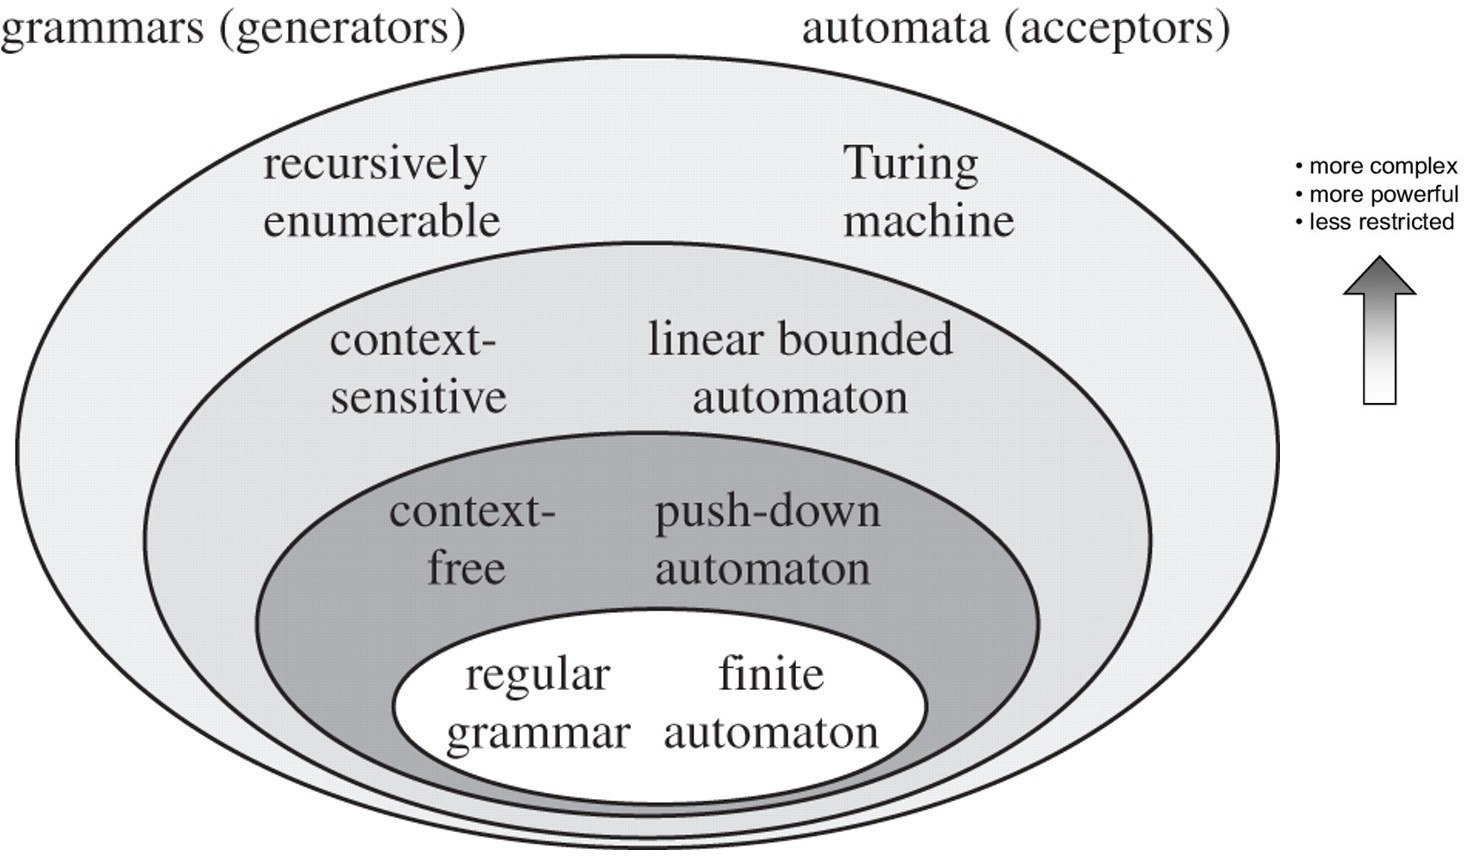
\includegraphics[width=0.8\textwidth]{chomsky}
    \caption{Hierarquia de Chomsky \cite{fitch}}
    \label{fig:chomsky}
\end{figure}

Uma gramática pode gerar uma linguagem possivelmente infinita, sendo assim, a
melhor maneira de representá-la é através da definição de um autômato.

Dentre os tipos de autômatos existentes, neste trabalho iremos abordar a
construção e o funcionamento das \emph{máquinas de estado finito} e das
\emph{máquinas de Turing}. Estes são responsáveis pelo reconhecimento das
\emph{gramáticas regulares } e \emph{recusivamente enumeráveis},
respectivamente.
